%%%%%%%%%%%%%%%%%%%%%%%%%%%%%%%
%%%%%%%%%%%%%%%%%%%%%%%%%%%%%%%
\chapter{Summary of papers}\label{ch:results}
\noindent This chapter presents a summary of the papers appended to this thesis, which includes research activities and a selection of the most relevant results. The relationships between the papers are summarized in \autoref{fig:papers}. The first two papers focus on the roll motion, in which the work conducted using Ikeda's method in Paper \ref{pap:rolldamping} is continued in Paper \ref{pap:ikeda}. 
The work exploring inverse dynamics that was initiated in the roll motion papers continued in the remaining manoeuvring papers.
Multicollinearity was found to be a significant challenge in Paper \ref{pap:pit}, and was initially addressed through model truncation.
However, model generalization may be reduced when model truncation is used, which was shown in Paper \ref{pap:physics}. Instead, the multicollinearity between the hull and rudder forces was mitigated by introducing a semi-empirical rudder model. The multicollinearity between the drift and yaw rate dependent forces was subsequently addressed in Paper \ref{pap:vct}. In addition, see \autoref{tab:objectives} in \autoref{sec:motivation} for a discussion of the relationship between these papers and the research objectives of this thesis.
\begin{figure}[h]
    
    \centering
    \begin{tikzpicture}[node distance = 1.5cm]
    
    \node (Paper1) [paper] {\footnotesize Paper 1};
    \node (Ikeda) [output, right of=Paper1, xshift=0] {\footnotesize Ikeda};
    \node (Paper2) [paper, right of=Ikeda] {\footnotesize Paper 2};
    \node (ID) [output, below of=Paper1, yshift=0.7cm] {\footnotesize inverse dynamics};
    \node (Paper3) [paper, below of=ID, yshift=0.7cm] {\footnotesize Paper 3};
    \node (multicollinearity) [output, below of=Paper3, yshift=0.7cm] {\footnotesize multicollinearity};
    \node (hull_vs_rudder) [output, below left of=multicollinearity, xshift=-0.5cm] {\footnotesize hull vs. rudder};
    \node (beta_vs_r) [output, below right of=multicollinearity, xshift=0.5cm] {\footnotesize $\beta$ vs. $r$};
    \node (Paper4) [paper, below of=hull_vs_rudder, , yshift=0.7cm] {\footnotesize Paper 4};

    \node (VCT) [output, below of=beta_vs_r, xshift=0, yshift=0.7cm] {\footnotesize VCT};
    \node (truncate) [output, above right of=beta_vs_r, xshift=0] {\footnotesize truncation};

    \node (Paper5) [paper, below of=VCT, , yshift=0.7cm] {\footnotesize Paper 5};

    %\draw[red, thick] ($(Paper1.north west)+(-0.25cm,0.25cm)$) rectangle ($(Paper2.south east)+(0.25cm,-0.25cm)$);
    %\draw[red, thick] ($(Paper3.north west)+(-2.15cm,0.25cm)$) rectangle ($(Paper5.south east)+(2.25cm,-0.25cm)$);

    
    \draw [decorate,decoration={brace,amplitude=5pt,mirror,raise=4ex}]
  (-2.5cm,0.25cm) -- (-2.5cm,-0.50cm) node[midway, rotate=90, yshift=1cm]{\footnotesize roll};
    
    \draw [decorate,decoration={brace,amplitude=5pt,mirror,raise=4ex}]
  (-2.5cm,-0.55cm) -- (-2.5cm,-5.25cm) node[midway, rotate=90, yshift=1cm]{\footnotesize manoeuvring};
    
    %Connect
    \draw [arrow] (Paper1) -- (Ikeda);
    \draw [arrow] (Ikeda) -- (Paper2);
    \draw [arrow] (Paper1) -- (ID);
    \draw [arrow] (ID) -- (Paper3);
    \draw [arrow] (Paper3) -- (multicollinearity);
    \draw [arrow] (multicollinearity) -| (hull_vs_rudder);
    \draw [arrow] (hull_vs_rudder) -- (Paper4);
    \draw [arrow] (multicollinearity) -| (beta_vs_r);
    \draw [arrow] (beta_vs_r) -- (VCT);
    \draw [arrow] (multicollinearity) -- (truncate);
    \draw [arrow] (truncate) |- (Paper3);
    \draw [arrow] (VCT) -- (Paper5);
    \draw [arrow] (ID.west) -- ++(-1.5cm,0cm) |-  (Paper5.west);
    
    \end{tikzpicture}
    \caption{Paper connections.}
    \label{fig:papers}
\end{figure}
%Section Comments: "Second generation intact stability criteria" seems more commonly used. It would help to specify a specific time period instead of saying "a long time."
\section{Summary of Paper \ref{pap:rolldamping}}
\subsection*{"\nameref{pap:rolldamping}"}
\subsection*{Scope and motivations}
The first step in this research project was to limit the system identification of the ship dynamics to only one degree of freedom. An accurate modeling of the roll motion is crucial, where 

\textcite{france_investigation_2001} demonstrated that the APL China casualty in 1998, where a post-Panamax C11 class container ship lost almost a third of its containers, was most likely caused by head sea parametric rolling.

was investigated in Paper \ref{pap:rolldamping} 

\subsection*{Results and concluding remarks}


System identification of ship roll motion, which includes roll damping and stiffness, is developed in Paper \ref{pap:rolldamping}. Parametric roll was observed by \textcite{froude_rolling_1861} and has been a focus of the marine research community since the early 1950s \parencite{galeazzi_early_2013}; it has received even more attention since \textcite{france_investigation_2001} demonstrated that the APL China casualty in 1998, where a post-Panamax C11 class container ship lost almost a third of its containers, was most likely caused by head sea parametric rolling. The damping of roll motion plays an important role in these phenomena. Previous literature demonstrates that the relatively small difference in the roll damping prediction obtained with small method variation may contribute to the difference between severe roll angles and much less noticeable motions \cite{soder_ikeda_2019}.

The objective of Paper \ref{pap:rolldamping} was to improve the roll damping predictions for modern ships. The roll damping was studied using time series data from 250 (see \autoref{fig:ship_types}) roll decay tests (see \autoref{sec:roll}) assembled by the Maritime Dynamics Laboratory at RISE SSPA Maritime center. The work was divided into the following sub tasks (also summarized in \autoref{fig:paper1_overview}): 
\vspace{5pt}
\begin{itemize}
    \setlength\itemsep{5pt}
    \item Find the mathematical model that is the best representation of the roll motion.
    \item Identify the parameters in this model for all the tests.
    \item Compare the identified parameters with state of art predictions.
    \item Develop a generic roll damping model for all ships using the identified parameters.
    \begin{itemize}
        \item Grey-box model
        \item Black-box model
    \end{itemize}
\end{itemize}
\vspace{5pt}
\begin{figure}[!htb]
    \centering
    \includegraphics[width=0.6\columnwidth]{kappa/images/ship_types.eps}
    \caption{Number of tests per ship type.}
    \label{fig:ship_types}
\end{figure}
\begin{figure}[!htb]
    \centering
\begin{tikzpicture}[node distance=3cm]
\node (data_collection) at (0,0) {Data collection:};
\node (roll_decay_DB) [database,label=below:Roll decay DB, right of=data_collection, xshift=-0.5cm]{};
\node (PIT) [process, right of=roll_decay_DB, xshift=0.5cm] {PIT};
\node (damping_DB) [database, label=below:Damping DB, right of=PIT, xshift=0cm] {};
\path (roll_decay_DB) -- node(time_series)[xshift=3.0cm]{Time series} -- (PIT);
\draw [arrow] (roll_decay_DB) -- (time_series) -- (PIT);
\path (PIT) -- node(B){B} (damping_DB);
\draw [arrow] (PIT) -- (B) -- (damping_DB);

\node (comparison)[below of=data_collection, yshift=0.5cm]{Comparison:};
%plot:
\node (origo)[right of=comparison, xshift=-0.5cm, yshift=-1cm];
\node(y)[above of=origo, yshift=-1cm]{Simplified ikeda};
\node(x)[right of=origo, xshift=-1cm]{Damping DB};
\draw[->](origo) -- (y);
\draw[->](origo) -- (x);
\draw node[anchor=south, right of=origo, xshift=-3cm, yshift=0cm] {\textbullet};
\draw node[anchor=south, right of=origo, xshift=-2.5cm, yshift=0.6cm] {\textbullet};
\draw node[anchor=south, right of=origo, xshift=-2cm, yshift=1cm] {\textbullet};
\draw node[anchor=south, right of=origo, xshift=-2cm, yshift=1.2cm] {\textbullet};
\draw node[anchor=south, right of=origo, xshift=-1.5cm, yshift=1.7cm] {\textbullet};
\draw node[anchor=south, right of=origo, xshift=-1.5cm, yshift=1.3cm] {\textbullet};
\draw node[anchor=south, right of=origo, xshift=-1cm, yshift=2cm] {\textbullet};

\node (regressions)[below of=comparison, yshift=-0.5cm]{Regressions:};
\node (damping_DB2) [database,label=below:Damping DB, right of=regressions, xshift=-0.5cm]{};
\node (grey_box) [grey-box, right of=damping_DB2, xshift=0.5cm, yshift=1.5cm] {Grey-box};
\node (black_box) [black-box, below of=grey_box, yshift=1.5cm] {Black-box};
\draw [arrow] (damping_DB2) |- (grey_box);
\draw [arrow] (damping_DB2) -- (black_box);
\end{tikzpicture}
    \caption{Overview of the work conducted for Paper \ref{pap:rolldamping}.}
    \label{fig:paper1_overview}
\end{figure}
System identification on the time series from the roll decay database was performed with the linear (\autoref{eq:roll_decay_equation_himeno_linear}), quadratic (\autoref{eq:roll_decay_equation_himeno_quadratic_b}), and cubic models (\autoref{eq:roll_decay_equation_cubic}). Estimated roll damping parameters were used to build a roll damping database. The database could be compared to corresponding predictions with the simplified Ikeda's method \cite{kawahara_simple_2011}, which is the state of art prediction for ship roll damping.
The generic roll damping model was developed as a grey-box model and a black-box model.
\subsection{Best mathematical model for the roll motion}
System identification on the linear, quadratic, and cubic models was conducted using both the \say{integration approach} (\autoref{sec:integration_approach}) and the \say{derivation approach} (\autoref{sec:derivation_approach}) where the best parameter estimations were obtained using the ``integration approach''.
Results from the simulations with the identified models (from one of the roll-decay tests) are presented in \autoref{fig:roll_decay_compare}. The cubic and quadratic models reproduce the model test well, and the linear model is too simple to provide an accurate representation for both smaller and larger roll angles. The amplitude decrement $\phi_a$ and roll damping $B$ for each oscillation can be visualized, as seen in \autoref{fig:roll_decay}.
\begin{figure}[h!]
    \centering
    \includegraphics[width=\linewidth]{kappa/images/roll_decay_model_compare.pdf}
    \caption{Roll decay estimation with identified cubic, quadratic, and linear models.}
    \label{fig:roll_decay_compare}
\end{figure}
\begin{figure}[h!]
    \begin{subfigure}[b]{0.45\textwidth}
        \centering
        \includegraphics[width=0.9\linewidth]{kappa/images/roll_decay_amplitude.pdf}
        \caption{Amplitude decrements.}
        \label{fig:roll_decay_amplitude}
    \end{subfigure}
        ~ %add desired spacing between images, e. g. ~, \quad, \qquad, \hfill etc. 
      %(or a blank line to force the subfigure onto a new line)
    \begin{subfigure}[b]{0.45\textwidth}
        \centering
        \includegraphics[width=0.9\linewidth]{kappa/images//roll_decay_damping.pdf}
        \caption{Dampings.}
        \label{fig:roll_decay_damping}
    \end{subfigure}
    \caption{Roll decay model test, linear-, quadratic- and cubic-model.}
    \label{fig:roll_decay}
\end{figure}
The goodness of fit for the linear, quadratic, and cubic models can be expressed using the coefficient of determination:
\begin{equation} \label{eq:R2}
%R^2=1-\frac{SS_{res}}{SS_{tot}}
R^2=1-\frac{\sum\limit_{i=1}^{n}(\phi_{i}-\hat{\phi}_i)^2}{\sum\limit_{i=1}^{n}(\phi_i-\bar \phi)^2}
\end{equation}
where $\phi_i$ is the model test roll angle at time step $i$, $\bar \phi$ is the mean roll angle from the model test, and $\hat{\phi}_i$ is the predicted roll angle (with the linear, quadratic, or cubic model). The average goodness of fit $R^2$ was 0.995 for the cubic model, 0.993 for the quadratic model, and 0.986 for the linear model. These values indicate that the quadratic model is almost as useful as the cubic model for describing the roll motion. The quadratic model, with fewer parameters than the cubic model, is expected to have a higher level of generalization at the same accuracy and is therefore selected as the best mathematical model for the roll motion. 

\subsection{Comparison with Ikeda's method}
The hydrodynamic analysis requires the ship's exact hull geometry. Building the geometry model and performing the strip-theory based hydrodynamic analysis are time-consuming. A ship's hull geometry is not always available for such purposes. A simplified Ikeda's method (SI-method) proposed by \textcite{kawahara_simple_2011} is used in Paper \ref{pap:rolldamping} to calculate all the damping components, which include the eddy component $B_E$ and the wave component $B_W$. The semi-empirical formulas describe four of the five roll damping components at motion frequency $\omega$ for a given roll amplitude $\phi_a$ at zero ship speed. A speed dependency was introduced by adding a fifth damping term $B_L$ and a speed correction to $B_W$ and $B_E$, as described in \textcite{ikeda_velocity_1979}, giving a function: 
\input{equations/simplified_ikeda_equation}

\noindent The formulas within $f$ can be expressed as \textcite{ikeda_velocity_1979, kawahara_simple_2011} with the implementation in \textcite{alexandersson_rolldecay-estimators_2022}.
It should be noted that this method is only efficient for the estimation of the roll damping of ships within the boundaries \parencite{kawahara_simple_2011}:
\begin{equation}
    \label{eq:SI_limits}
     \left\{
     \begin{array}{ll}
    0.5 \leq C_b \leq 0.85,\hspace{0.5cm} 
    0 \leq \hat{\omega} \leq 1.0,
    \hspace{0.5cm}
    0.9 \leq A_0 \leq 0.99,\\
    2.5\leq Beam/T \leq 4.5, \hspace{1cm}
    0.01 \leq BK_B/Beam \leq 0.06, \\
        -1.5 \leq OG/T \leq 0.2,
     \hspace{1cm}
    0.05 \leq BK_L/L_{PP} \leq 0.4.
    \end{array}
    \right.
\end{equation}

\noindent The total roll damping is predicted as the sum (\autoref{eq:ikeda}) of the damping contributions (\autoref{eq:simplified_ikeda_equation}). This damping can be compared with the linearized equivalent damping $B_e$, which is calculated for a certain roll angle $\phi_a$ with the identified roll damping parameters $B_1$ and $B_2$ \cite{himeno_prediction_1981},
\input{equations/B_e_equation}

\noindent The $B_e$ non-dimensional form of the coefficient can be used according to \textcite{himeno_prediction_1981}. The non-dimensional equivalent for the linear damping coefficient is $\hat{B_e}$. This form is more convenient when comparing roll damping for different ships,
\begin{equation} \label{eq:be_eqvalent}
    \hat{B_e} = \frac{B_e}{\rho \bigtriangledown Beam^2} \sqrt{\frac{Beam}{2g}},
\end{equation}
\noindent where $\rho$, $\bigtriangledown$, and $Beam$ stand for fluid density, displacement volume, and breadth of a ship, respectively. Prediction error plots of $\hat{B_e}$ from the simplified Ikeda's method and identified damping from the model tests are presented in \autoref{fig:si_model_within}. In this figure, a comparison of predictions with roll amplitudes in the range of 0 to 10 degrees is displayed for all ships with no limits and for ships within the limits of the method (\autoref{eq:SI_limits}). The $R^2$ values of the predictions are displayed in \autoref{tab:si_validation}. There is reasonable agreement between the predicted roll damping and model tests for ships within the limits. There is very poor agreement for ships outside the limits. It should be noted that most of the points are outside the limits of the method.

\begin{figure}[h!]
\centering
    \begin{subfigure}[b]{0.45\textwidth}
    
        \centering
        \includegraphics[width=\textwidth]{kappa/images/si_model_within.pdf}
        %\vspace{-0.5cm}
        \caption{The simplified Ikeda's method within and outside its limits.}
        \label{fig:si_model_within}
    \end{subfigure}
    \hfill
    \begin{subfigure}[b]{0.45\textwidth}
        \centering
        \includegraphics[width=\textwidth]{kappa/images/component_residual.pdf}
        \vspace{-0.2cm}
        \caption{Residuals vs. components.}
        \label{fig:component_residual}
        \vspace{0.3cm}
    \end{subfigure}
    \hfill
    \begin{subfigure}[b]{0.45\textwidth}
        \centering
        \includegraphics[width=\textwidth]{kappa/images/si_ikeda_model.pdf}
        \caption{Comparison of simplified and original Ikeda's method and model tests.}
        \label{fig:si_ikeda_model}
    \end{subfigure}

    \caption{Prediction error plots.}
\end{figure}
\input{equations/si_validation}
\noindent The largest contribution to the error in the predictions comes from the wave damping $B_W$, as seen in \autoref{fig:component_residual}. A comparison of the simplified Ikeda's method and the original Ikeda's method was carried out in Paper \ref{pap:rolldamping}; the comparison was used to determine whether the observed deviations are the result of extrapolation or inherent to the original method. In Ikeda's method, more extensive knowledge of the ship hull geometry is needed in order for $B_W$ to be calculated with a strip method and $B_E$ to be calculated with sectional Lewis coefficients. It was possible to collect the required hull inputs for 15 ships in the database. These ships were used in 50 of the reference roll decay tests; all but one of the tests exceed the limits. Ikeda's method has much more agreement for these exceeding model tests according to \autoref{fig:si_ikeda_model} and the calculated $R^2$ in Table \ref{tab:si_ikeda_validation}.

\input{equations/si_ikeda_validation}
\subsection{Generic roll damping model}
\label{sec:genericrolldampingmodel}
A serial grey-box model for ship roll damping (see \autoref{fig:greyrolldamping}) is also developed in Paper \ref{pap:rolldamping}. 
This is expanding the system identification by not only focusing on one ship, but all modern ships. 
The simplified Ikeda's method \cite{kawahara_simple_2011} is used as the white-box model, which is combined with the following black-box correction model.

\begin{figure}[H]
    
    \centering
    \begin{tikzpicture}[node distance=2cm]
    \node (white-box) [white-box] {\footnotesize Simplified Ikeda};
    \node (B_BK) [io, right of=white-box, xshift=0.90cm, yshift=1.5cm] {\footnotesize $\hat{B_{BK}}$};
    \node (B_E) [io, right of=white-box, xshift=0.75cm, yshift=0.75cm] {\footnotesize $\hat{B_{E}}$};
    \node (B_F) [io, right of=white-box, xshift=0.75cm, yshift=0cm] {\footnotesize $\hat{B_{F}}$};
    \node (B_L) [io, right of=white-box, xshift=0.75cm, yshift=-0.75cm] {\footnotesize $\hat{B_{L}}$};
    \node (B_W) [io, right of=white-box, xshift=0.75cm, yshift=-1.5cm] {\footnotesize $\hat{B_{W}}$};
    
    
    \node (black-box) [black-box, right of=B_F, xshift=0.75cm] {\footnotesize Black-box};
    \draw [arrow] (white-box) -- (B_BK);
    \draw [arrow] (white-box) -- (B_E);
    \draw [arrow] (white-box) -- (B_F);
    \draw [arrow] (white-box) -- (B_L);
    \draw [arrow] (white-box) -- (B_W);
    
    \draw [arrow] (B_BK) -- (black-box);
    \draw [arrow] (B_E)  -- (black-box);
    \draw [arrow] (B_F)  -- (black-box);
    \draw [arrow] (B_L)  -- (black-box);
    \draw [arrow] (B_W)  -- (black-box);
    
    
    \node (B) [io, right of=black-box, xshift=0.75cm, yshift=0cm] {\footnotesize $B$};
    \draw [arrow] (black-box)  -- (B);
    
    \end{tikzpicture}
    \caption{Grey-box model to predict roll damping.}
    \label{fig:greyrolldamping}
\end{figure}

\noindent The roll damping data set, obtained from the roll motion investigation, is intended to train the black-box component of the grey-box model. The black-box correction model of the output components from the simplified Ikeda's method is displayed in (\autoref{eq:polynom_correction}),
\input{equations/polynom_correction}

\noindent Major corrections to the skin friction damping $\hat{B_F}$ and wave damping $\hat{B_W}$ are included in this expression. The corrections are included because the simplified Ikeda's method is not very accurate for this dataset; most of the ships in the dataset exceeded the limits of the method. A pure black-box model is also developed in Paper \ref{pap:rolldamping} (see \autoref{eq:polynom_complex}),
\input{equations/polynom_complex}
\noindent where non-dimensional frequency $\hat{\omega_0}$ is calculated with \autoref{eq:omega0_hat_equation} \cite{himeno_prediction_1981},
\input{equations/omega0_hat_equation}
Over-fitting data is a concern when constructing a regression model from a data set. Including too many parameters or allowing the order of the model to be too high would provide a very accurate representation of the present roll damping data. However, such a representation would be accompanied by major extrapolation errors when the model is used for other data. The generalization of the model can be assessed with a hold-out evaluation by using K-fold cross validation \cite{mosteller_handbook_1968} (\autoref{fig:k-fold}).\input{kappa/fig_k-fold} The data has been divided into five smaller sets (folds). Four of the folds are used to train the model, and the fifth fold is used for testing (validation). Validation consists of calculating the coefficient of determination $R^2$ for the fitted model. Validation is completed for all five possible train-test combinations. 
The folds are randomly constructed with the restriction that all data for a particular ship must be in the same fold. Five folds are randomly generated 20 times, which gives 100 values of $R^2$ from the train-test-procedure for each model. The mean values and standard deviation of these 100 values of $R^2$ are displayed in Table \ref{tab:crossvalidation}. The mean and standard deviation of $R^2$ simplified Ikeda's method in this table were calculated directly instead of using cross validation because they do not rely on the SSPA data.
\input{equations/cross_validation}
\clearpage
\section{Summary of Paper \ref{pap:ikeda}}
\subsection*{"\nameref{pap:ikeda}"}
\subsection*{Scope and motivations}
An explicit semi-empirical formula was proposed in Paper \ref{pap:rolldamping}, based on the simplified Ikeda's method \cite{kawaharaSimplePredictionFormula2011}. This is an alternative with very low computational cost. However, it was also found to have poor accuracy, especially for modern ship designs. 
Paper \ref{pap:ikeda} proposed a new hybrid method, as a solution to this problem, where the viscous roll damping from Ikeda’s semi-empirical method was injected into an existing 3D unsteady fully nonlinear potential flow (FNPF) method \cite{kjellbergFullyNonlinearUnsteady2013}.

\subsection*{Results and concluding remarks}
The viscous roll damping was calculated with Ikeda's method \cite{ikedaComponentsRollDamping1978} for the KVLCC2 test case. Error in the calculation of the $C_r$ coefficient to obtain the eddy damping at zero speed was encountered, which was found to originate from a regression formula from experiments conducted by \textcite{ikedaEddyMakingComponent1978} on a number of two-dimensional cylinders with various sections. A new regression was instead proposed, using a decision tree model.
Fig.\ref{fig:ikeda_sections} shows $C_r$ from the experiments and corresponding predictions with Ikeda's method and the decision tree. The capital letters refer to cylinder sections from the experiments
\cite{ikedaEddyMakingComponent1978}.
\begin{figure}[h]
\center
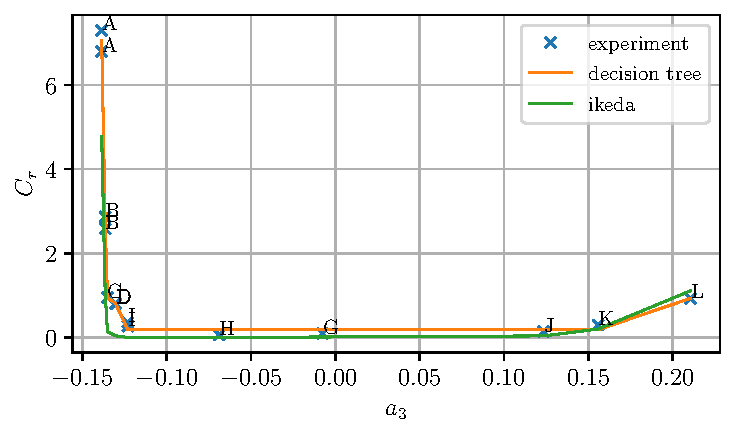
\includegraphics[width=\textwidth]{figures/ikeda_sections.pdf}
\vspace{-0.4cm}
\caption{$C_r$ for cylinder sections from experiments and predicted with Ikeda's method and the decision tree model.}
\label{fig:ikeda_sections}
\end{figure}
\FloatBarrier

The total predicted roll damping was reasonably in good agreement with the damping of the model tests at zero speed (\autoref{fig:hybrid_0}) and very well in agreement at speed (\autoref{fig:hybrid_speed}).
\begin{figure}[h]
\begin{center}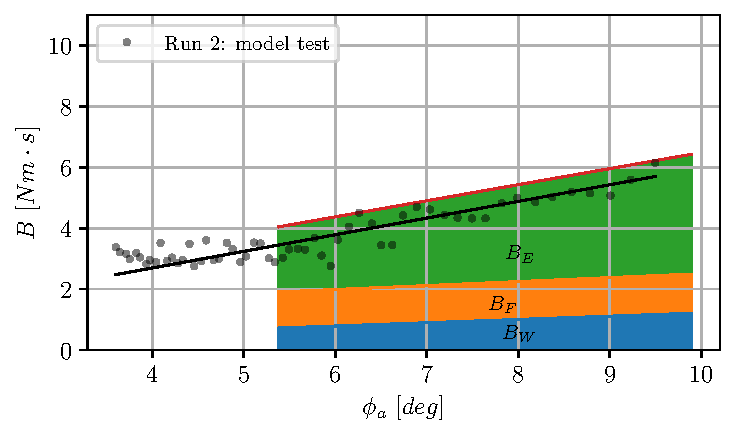
\includegraphics[width=\textwidth]{figures/hybrid_0.pdf}\end{center}
%\vspace{-0.4cm}
\caption{Roll damping from hybrid method ($F_n = 0$) for KVLCC2.}
\label{fig:hybrid_0}
\end{figure}
\begin{figure}[h]
\begin{center}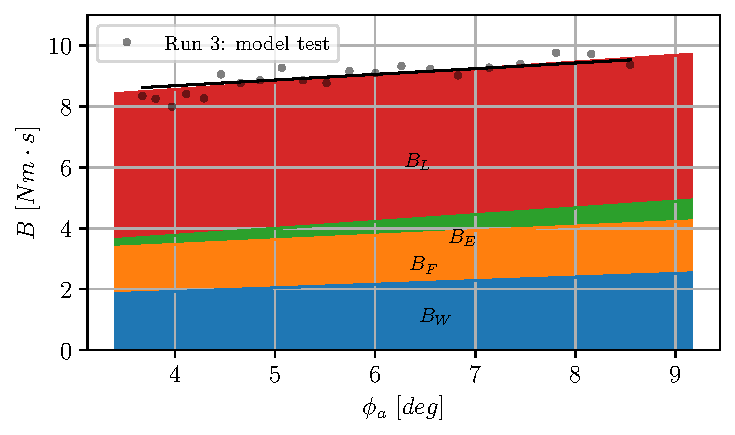
\includegraphics[width=\textwidth]{figures/hybrid_speed.pdf}\end{center}
%\vspace{-0.4cm}
\caption{Roll damping from hybrid method ($F_n = 0.14$) for KVLCC2.}
\label{fig:hybrid_speed}
\end{figure}
Roll decay simulations with damping from the hybrid method were conducted. Results from these simulations were compared with the model tests at zero speed (\autoref{fig:hybrid_0_time}) and at speed (\autoref{fig:hybrid_speed_time}). The time series from the corresponding FNPF
simulations have also been added to these plots to show how much the injection of semi-empirical viscous damping can improve the accuracy of these simulations.

Paper \ref{pap:ikeda} concluded that Ikeda's method offers an effective semi-empirical approach for predicting viscous roll damping. When combined with modern potential flow codes like FNPF, it enables highly accurate predictions of ship roll motion 
\begin{figure}[h]
\center
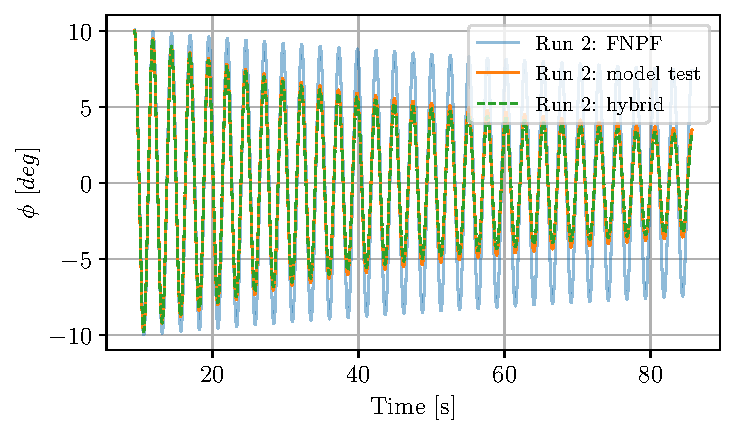
\includegraphics[width=\textwidth]{figures/hybrid_0_time.pdf}
%\vspace{-0.7cm}
\caption{Roll decay ($F_n=0$) for KVLCC2.}
\label{fig:hybrid_0_time}
\end{figure}
\begin{figure}[h]
\center
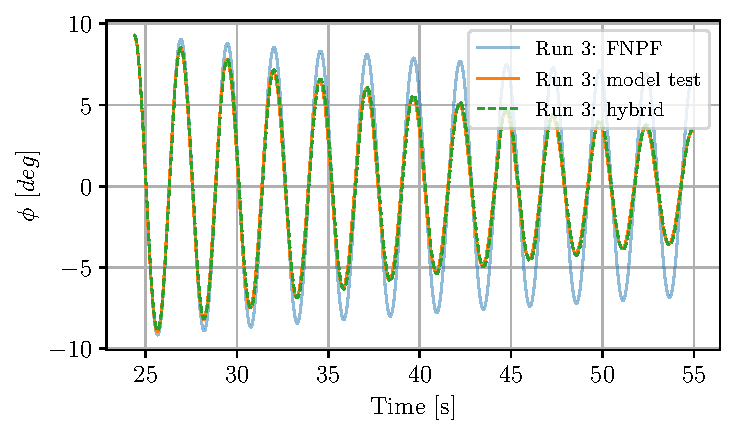
\includegraphics[width=\textwidth]{figures/hybrid_speed_time.pdf}
%\vspace{-0.7cm}
\caption{Roll decay ($F_n=0.14$) for KVLCC2.}
\label{fig:hybrid_speed_time}
\end{figure}
\section{Summary of Paper \ref{pap:pit}}
\subsection*{"\nameref{pap:pit}"}
\subsection*{Scope and motivations}
In order to expand the modeling complexity and uncertainty from Paper \ref{pap:rolldamping}, system identification of manoeuvring by adding the the surge, sway, and yaw degrees of freedom was studied in Paper \ref{pap:pit}. 
The objective was to find parametric model structures with good generalization and to develop parameter identification techniques from FRMT data.

The dynamics were assumed to be described by an Abkowitz or truncated Abkowitz model. 
The system identification method proposed in Paper \ref{pap:pit} was validated on two case study ships: the wPCC and the KVLCC2 (\autoref{fig:kvlcc2_hsva}). The parameters were identified with recursive inverse dynamics regression (see \autoref{sec:RIDR}).
The identification was carried out with cross validation using hold-out evaluation \cite{sammutHoldoutEvaluation2017}.
The data in this evaluation were divided into three sets: the training set, the validation set and the test set as seen in \autoref{fig:model_development_process}.
The purpose of the training set was to train all the candidate models using the proposed parameter estimation method. The validation set was used to select the most effective candidate model. The training and validation sets were joined to train the selected model as the final model. The final model was used for predicting the test set, which was used to evaluate the accuracy of the model. These three sets were not divided randomly;  they were divided to assess the model’s extrapolation ability. The data sets were therefore split to have the smallest yaw rates, drift-angles, and rudder-angles in the training set; the medium values in the validation set; and the largest values in the test set.
Examples of this can be seen for the two test cases in \autoref{fig:wpcc_datasets} and \autoref{fig:kvlcc2_datasets}.
%\begin{figure}[h!]
%\centering
%\includegraphics[width=0.5\linewidth]{kappa/images/wpcc_mdl.png}
%\caption{wPCC tested at SSPA Maritime center. Copyright 2020 by RISE.}
%\label{fig:wpcc-mdl}
%\end{figure}
\begin{figure}[h!]
    \centering
    \begin{subfigure}[b]{0.45\textwidth}
    \centering
    \includegraphics[height=3cm]{kappa/images/kvlcc2_front.png}
    \end{subfigure}
    ~
     \begin{subfigure}[b]{0.45\textwidth}
     \centering
     \includegraphics[height=3cm]{kappa/images/kvlcc2_aft.png}
     \end{subfigure}
+    \caption{Ship model used in HSVA and MARIN model tests. Copyright HSVA.}
    \label{fig:kvlcc2_hsva}
\end{figure}
\begin{figure}[H]
\centering
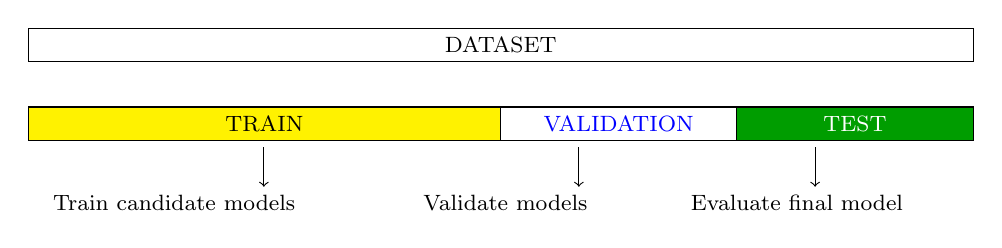
\begin{tikzpicture}

\node (dataset)[rectangle,
    anchor=west,
    draw,
    text = black,
    minimum width=12cm,
    fill = white] at (0, 0) {\footnotesize DATASET};

\node (train)[rectangle,
    draw,
    anchor=west,
    text = black,
    minimum width=6cm,
    fill = yellow] at (0, -1cm) {\footnotesize TRAIN};

\node (validation)[rectangle,
    draw,
    anchor=west,
    text = blue,
    minimum width=3cm,
    fill = white] at (6cm, -1cm) {\footnotesize VALIDATION};

\node (test)[rectangle,
    draw,
    anchor=west,
    text = white,
    minimum width=3cm,
    fill = black!15!green!255] at (9cm, -1cm){\footnotesize TEST};
    
\node (train_multiple)[rectangle,
    draw,
    anchor=west,
    text = black,
    draw = none,
    fill = none] at (0.2cm, -2cm){\footnotesize Train candidate models};
    
\node (validate_models)[rectangle,
    draw,
    anchor=west,
    text = black,
    draw = none,
    fill = none] at (4.9cm, -2cm){\footnotesize Validate models};
    
\node (evaluate_models)[rectangle,
    draw,
    anchor=west,
    text = black,
    draw = none,
    fill = none] at (8.3cm, -2cm) {\footnotesize Evaluate final model};

\draw[->] (3,-1.3) -- (3,-1.8);
\draw[->] (7,-1.3) -- (7,-1.8);
\draw[->] (10,-1.3) -- (10,-1.8);
\end{tikzpicture}
\caption{Model development process with hold-out evaluation.}
\label{fig:model_development_process}
\end{figure}
\begin{figure}[h!]
\centering
\includegraphics[width= 1.0\linewidth]{kappa/images/3.pdf}
\caption{wPCC training, validation and testing datasets.}
\label{fig:wpcc_datasets}
\end{figure}
\begin{figure}[h!]
\centering
\includegraphics[width=1.0\textwidth]{kappa/images/4.pdf}
\caption{KVLCC2 training, validation and testing datasets.}\label{fig:kvlcc2_datasets}
\end{figure}

\subsection*{Results and concluding remarks}
\autoref{fig:validation-forces} shows predictions of the wPCC validation set with the identified models. AVMM is a full Abkowitz model and MAVMM is a truncated Abkowitz model where model structure selection has been applied. The AVMM model over-predicted the forces by far. 
This over-prediction was  explained by the high multicollinearity of the AVMM model structure for the wPCC data as shown in \autoref{fig:ncorr}  where the absolute correlation coefficient between the features in the wPCC yaw moment regression is presented.
Therefore, simulations of the validation cases were only possible using the MAVMM. 
The MAVMM model was retrained on the joined test and validation data set to obtain the final prediction model which was used to predict the turning circle test data set as shown in \autoref{fig:track-plot-testing-sim}. Advance and tactical diameter \cite{imoStandardsShipManoeuvrability2002} from the prediction differs by 4\% and 1\%. Monte Carlo simulations with alternative realizations of the regression, considering the uncertainty in the regressed parameters, are also displayed in these figures. The alternative realizations have similar simulation results to the model with mean values of the regression (black line).
\begin{figure}[h]
\centering
\includegraphics[width=1.0\textwidth]{kappa/images/7.pdf}
\caption{Validation of force models for wPCC ZigZag20/20.}\label{fig:validation-forces}
\end{figure}
\begin{figure}[h]
\centering
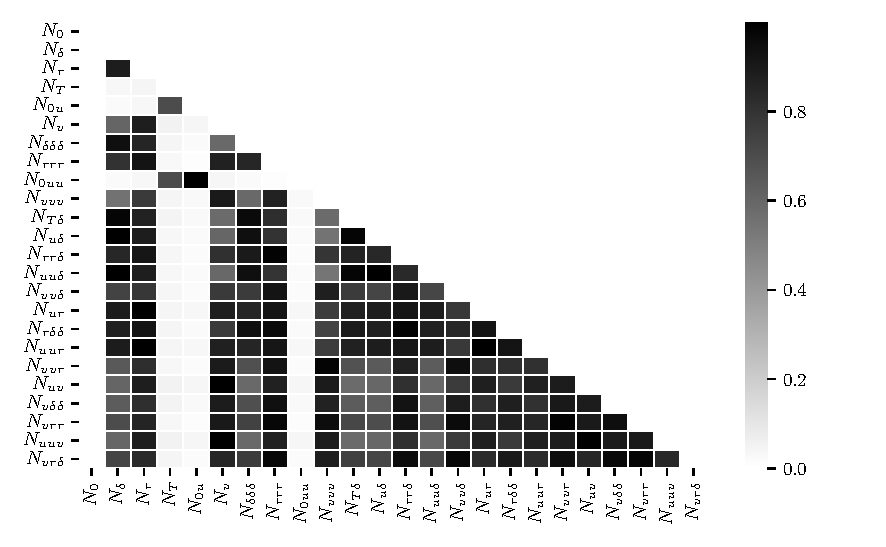
\includegraphics[width=1.0\textwidth]{kappa/images/10.pdf}
\caption{Absolute correlation between the features in the wPCC yaw moment regression of AVMM.}\label{fig:ncorr}
\end{figure}
\begin{figure}[h]
    \centering

    \begin{subfigure}[b]{\textwidth}
        \includegraphics[width=0.90\textwidth]{kappa/images/11.pdf}
        \caption{Track plots.}\label{fig:track-plot-testing-sim}
    \end{subfigure}
    \vfill
    \begin{subfigure}[b]{\textwidth}
        \includegraphics[width=0.90\textwidth]{kappa/images/12.pdf}
        \caption{Time series.}\label{\detokenize{06.10_results_wpcc:fig-testing-sim}}
    \end{subfigure}
        
    \caption{Turning circle test case for wPCC from model test and simulations.}
    \label{fig:enter-label}
\end{figure}

%\includegraphics[width=0.90\textwidth]{kappa/images/11.pdf}
%\caption{Turning circle test case for wPCC, track plots from model test and simulation.}\label{fig:track-plot-testing-sim}
%\end{figure}
%\begin{figure}[ht]
%\centering
%\includegraphics[width=0.90\textwidth]{kappa/images/12.pdf}
%\caption{Turning circle test case for wPCC, time series from model test and simulation.}\label{\detokenize{06.10_results_wpcc:fig-testing-sim}}\end{figure}
\FloatBarrier

The corresponding final prediction of the turning circle test for the KVLCC2 test case is shown in \autoref{fig:fig-kvlcc2-track-plot-testing-sim}. The prediction was conducted using simulation with the MAVMM trained on the training and validation datasets. Monte Carlo simulations with alternative realizations of the regression are also displayed in this figure. The alternative realizations are very similar to the model with mean values of the regression (black line).
The predicted advance and tactical diameters differ by 2\% and 5\%.
\begin{figure}[h]
    \centering

    \begin{subfigure}[b]{0.80\textwidth}
        \includegraphics[width=\textwidth]{kappa/images/17.pdf}
        \caption{Track plots.}
    \end{subfigure}
    \vfill
    \begin{subfigure}[b]{0.80\textwidth}
        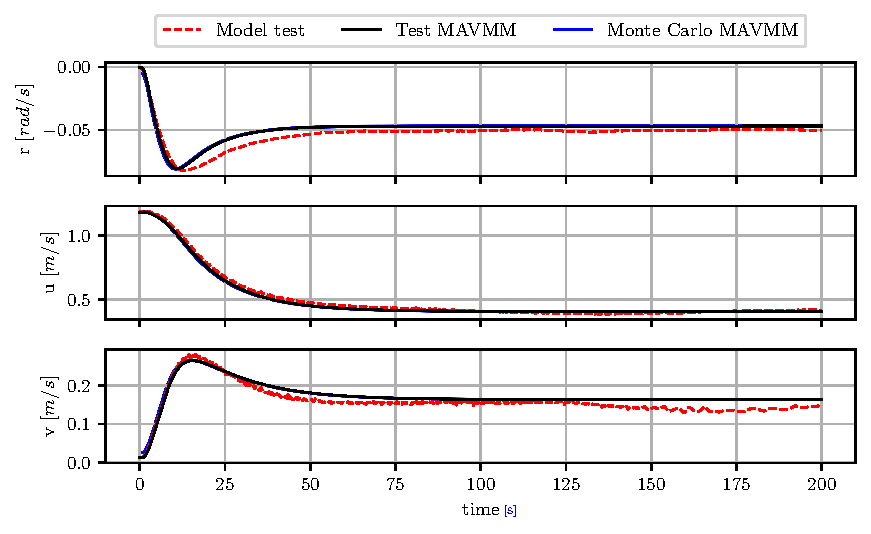
\includegraphics[width=\textwidth]{kappa/images/18.pdf}
        \caption{Time series}
    \end{subfigure}
        
    \caption{Comparison between the predicted turning circle test with MAVMM trained on HSVA data and MARIN model test results for KVLCC2.}
    \label{fig:fig-kvlcc2-track-plot-testing-sim}
\end{figure}
\section{Summary of Paper \ref{pap:physics}}
\subsection*{"\nameref{pap:physics}"}
\subsection*{Scope and motivations}
Minimizing the number of derivatives is often a good idea to avoid overfitting irrelevant data, following the prejudice approach that ''Nature is simple'' \cite{ljungPerspectivesSystemIdentification2010}. However, this could also lead to model structures with limited applicability, as certain regression terms may only become significant in special conditions like sailing in wind \cite{abkowitzMEASUREMENTHYDRODYNAMICCHARACTERISTICS1980}.

It was shown in Paper \ref{pap:pit} that it is possible to identify a model from calm water free running model test with inverse dynamics regression (\autoref{sec:IDR}) together with a cross validation technique to ensure good generalization so that the model can predict other kinds of maneuvers with very good accuracy. However, it was soon discovered that these models did not generalize well when wind forces were added to the simulations. This problem was addressed in Paper \ref{pap:physics}.

Paper \ref{pap:physics} uses two modular manoeuvring models. One of the models is a physics uninformed (PU) model which was a completely data driven model, similarly to the models used in the previous paper (Paper \ref{pap:pit}).
The other model was a physics informed (PI) model, where prior knowledge about rudder hydrodynamics has been added to guide the identification towards a more physically correct model. 
The models had identical prediction models for the hull and propeller forces but different models for the rudder forces. The PI model had a deterministic semi-empirical rudder model. The PU model had a data-driven mathematical rudder model. Except for the changed rudder models, the ship manoeuvring models were similar to the MMG model \cite{yasukawaIntroductionMMGStandard2015}, with some minor enhancements; The surge velocity was for instance expressed as a perturbed velocity (see \autoref{sec:prime_system}) allowing for higher order resistance coefficients.

A brief description of the workflow of Paper \ref{pap:physics} is shown in \autoref{fig:methodology}.
The PI and PU models were identified in free-running model tests using inverse dynamics and regression. To assess physical correctness, a reference model was established, where the PI model was instead identified on a VCT data set. This reference model, based on CFD, was assumed to be a sufficiently correct representation of the ship's physics.
Verification and comparisons between the models were carried out in the free-sailing model tests.
\begin{figure}[h]
  \centering
  %\includesvg[width=\columnwidth, pretex=\scriptsize, height=12cm]{figures/methodology2.svg}
  \includesvg[width=0.8\textwidth, pretex=\centering\fontsize{7.5}{8}]{kappa/images/methodology2.svg}
  \caption{Research workflow, describing how the reference model is identified with regression of VCT data and the PI and PU models are identified with regression of inverse dynamics forces from model tests. Results are then gathered to assess the parameter drift, physical correctness and generalization of the models.}
  \label{fig:methodology}
\end{figure}
It was investigated if the introduction of a deterministic semi-empirical rudder model in the PI model would reduce the multicollinearity and enhance the generalization.

\FloatBarrier
\clearpage
\subsection*{Results and concluding remarks}
Force predictions using reference, PI, and PU models for the states during one of the zigzag10/10 tests with wPCC were compared with the inverse dynamics forces for the same test in \autoref{fig:ID_zigzag10}. The PI and PU models predicted the same total yawing moment $N_D$ and sway force $Y_D$ as the reference model. However, the decomposition of this total yawing moment into components of the hull $N_H$ and the rudder $N_R$ differed significantly between the PU model and the PI and reference models, which were quite similar to each other.

\begin{figure}[h] \centering 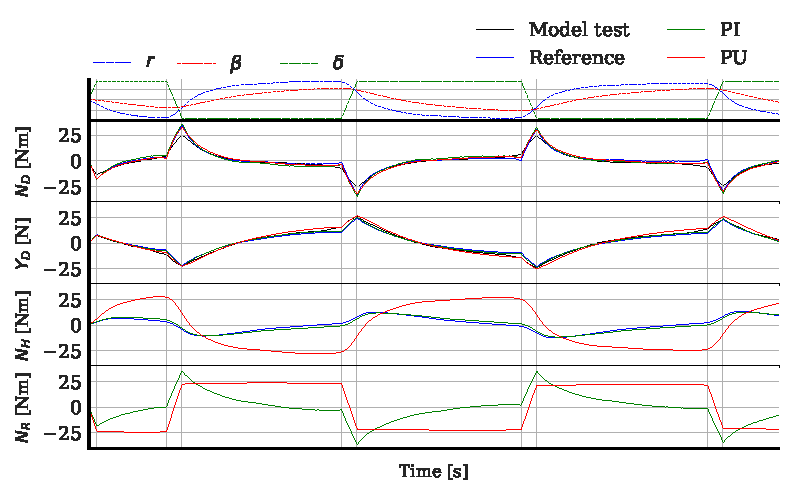
\includegraphics[width=0.9\textwidth]{kappa/images/results.ID_zigzag10.pdf} \caption{ID estimations of $Y_D$ and $N_D$ during a zigzag10/10 model test compared with model predictions.} \label{fig:ID_zigzag10} \end{figure}

The hull forces can be further decomposed into contributions from the drift of the vessel, through the sway velocity $v$, and contributions from the yaw rate $r$, as shown in \autoref{fig:ID_regression_N_decomposition}. It appears that almost all the yawing moments $N_H$ depend on $r$ for the PU model, and almost all the sway force $Y_H$ is generated by $v$. This contrasts with the other two models, where both $v$ and $r$ contribute to $N_H$ and $Y_H$.

\begin{figure}[h] \begin{center} \includesvg[width=0.9\textwidth]{kappa/images/results.hull_force_decomposition_zigzag20.svg} \caption{Decomposition of hull forces and moments during a zigzag20/20 test for parameters related to drift, yaw rate, and the prediction models.} \label{fig:ID_regression_N_decomposition} \end{center} \end{figure}

Thus, the PU model not only has an incorrect decomposition between rudder and hull forces, but it also incorrectly decomposes the drift and yaw rate contributions within the hull force model. However, this is not a significant problem during the zigzag tests, where the drift and yaw rate are highly correlated, as seen from the phase plot in \autoref{fig:phase_portrait}. This correlation can also explain why the completely data-driven model from the previous paper (Paper \ref{pap:pit}) achieves such good results despite the erroneous decomposition.

\begin{figure}[h] \centering \includesvg{figures/multicollineraity.multicollinearity.svg} \caption{Phase portrait showing the combination of drift angle and yaw rate for zigzag10/10 and zigzag20/20 wPCC model tests.} \label{fig:phase_portrait} \end{figure}

However, when the ship is exposed to wind, causing changes in drift, the erroneous decomposition of the PU model becomes apparent, as shown in \autoref{fig:result_wind_state}. The PI model aligns better with the reference model in the wind state. Introducing a semi-empirical rudder model seems to have guided the identification toward a more physically accurate model, with lower multicollinearity and better generalization from calm water zigzag tests to wind conditions.

\begin{figure}[h!] 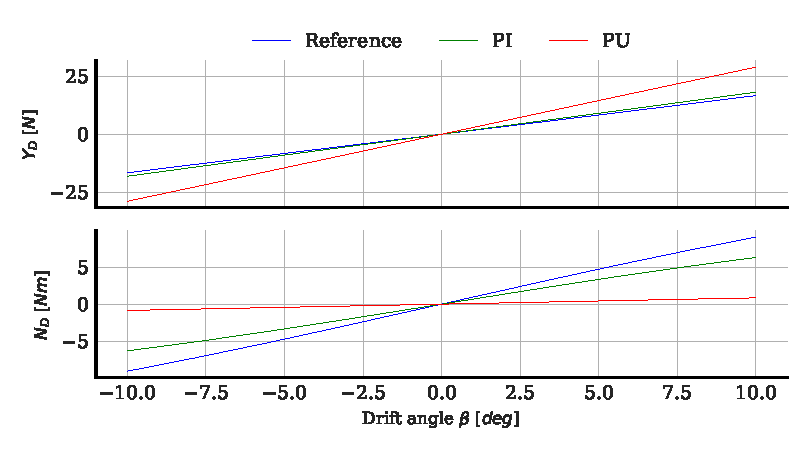
\includegraphics[width=\textwidth]{kappa/images/result_wind_state.forces.pdf} \caption{Total sway force and yawing moment from the wPCC models at various drift angles.} \label{fig:result_wind_state} \end{figure}

\FloatBarrier \clearpage
\section{Summary of Paper \ref{pap:vct}}
\subsection*{"\nameref{pap:vct}"}
\subsection*{Scope and motivations}
The objective of paper \ref{pap:vct} was to propose a parametric model structure based on physical insights from VCT and FT inverse dynamics. The reference model from Paper \ref{pap:physics} was assumed to be close to the physically correct true model of ship manoeuvring dynamics. This model was developed with VCT, which is based on physical first principles through CFD calculations. Paper \ref{pap:vct} investigated the identification of manoeuvring with VCT more closely, with the aim of achieving a model that more accurately reflected the true system.

Manoeuvring models were developed for the two WAPS test cases with large rudders. The models were identified by conducting a VCT to obtain hydrodynamic damping coefficients and by conducting pure yaw and pure sway tests in FNPF to obtain the added masses using the Fourier series method (see \autoref{sec:fourier}). The identified force models were compared with the inverse dynamics forces of the zigzag tests to identify potential weaknesses within the models.

\subsection*{Results and main findings}
Propeller and rudder forces were measured during the FRMTs for Optiwise. It was found that these measured forces together with forces predicted with a hull sub module, identified from VCT data, could recreate the estimated inverse dynamics forces during zigzag maneuvers with sufficient accuracy. Much effort was therefore devoted to finding a rudder force prediction model that could recreate the rudder forces for Optiwise. A modified quadratic MMG rudder model was proposed (see \autoref{sec:MMG_rudder}) as an improved version of the original model \cite{yasukawaIntroductionMMGStandard2015}. 
\autoref{fig:MMG_quadratic} shows the Optiwise rudder force $Y_R$ for the various VCT test types (see \autoref{sec:VCT}) plotted against the effective rudder angle $\beta_R$. The original MMG rudder model has a constant flow straightening factor $\gamma_{Rpos}$ for positive $\beta_R$ and another constant flow straightening factor $\gamma_{Rneg}$ for negative $\beta_R$. The proposed quadratic formulation has two additional parameters, $\gamma_{R2pos}$ and $\gamma_{R2neg}$, that allow the flow straightening to vary with $\beta_R$ that better fits the VCT data.
\begin{figure}[h]
     \centering
     \begin{subfigure}[b]{0.49\textwidth}
         \centering
         \includesvg[width=1\textwidth]{figures/results_optiwise_VCT.Y_R_MMG_original.svg}
        \caption{Original MMG rudder model.}
        \label{fig:Y_R_MMG_original}
     \end{subfigure}
     \hfill
     \begin{subfigure}[b]{0.49\textwidth}
         \centering
         \includesvg[width=1\textwidth]{figures/results_optiwise_VCT.Y_R_MMG_quadratic.svg}
        \caption{Modified quadratic MMG rudder model.}
        \label{fig:Y_R_MMG_quadratic}
     \end{subfigure}
    \caption{Rudder force during the VCT tests as a function of the effective inflow angle for the original MMG model and the modified quadratic MMG model.}
    \label{fig:MMG_quadratic}
\end{figure}

The rudder forces during the Optiwise FRMTs were predicted and compared with the corresponding measured forces, as shown in \autoref{fig:rudder_forces}. Although there were some minor deviations during the zigzag10/10 test, there was generally good agreement between the predictions and measurements. VCT calculations of some of the states during the manoeuvres have also been added to this comparison, which also show good agreement.
\begin{figure}[h]
    \centering
    \begin{subfigure}[b]{\textwidth}
        \centering
        \includesvg{figures/results_optiwise_ID.rudder_forces_zigzag 10_10.svg}
        \caption{Zigzag10/10 to port.}
        \label{fig:ID_measured_rudder_zigzag_10_10}
    \end{subfigure}
     \vfill
    \begin{subfigure}[b]{\textwidth}
        \centering
        \includesvg{figures/results_optiwise_ID.rudder_forces_zigzag 20_20.svg}
        \caption{Zigzag20/20 to starboard.}
        \label{fig:ID_measured_rudder_zigzag_20_20}
    \end{subfigure}
    \caption{Rudder forces during the zigzag tests compared to predictions with the MMG models.}
    \label{fig:rudder_forces}
\end{figure}

The total forces during the zigzag tests were also predicted, including the hull and rudder models. \autoref{fig:ID_optiwise20}  shows a comparison between the predicted forces and FRMT inverse dynamics forces. VCT calculations of some of the states during the manoeuvres have also been added to this figure, which agrees well with the model predictions.
However, deviations were observed for the sway force $Y_D$ within three seconds after the rudder changes at t = 11--14 s and t = 35--38 s, for the zigzag10/10 and t = 11--14 s, t = 35--38 s, t = 64 s, for the zigzag20/20. The model and state VCT calculations predict a straighter line in the $Y_D$ time series near these deviation points. No reasonable explanation for these deviations has been found, and filtration errors in the EKF were ruled out as a possible explanation.
\begin{figure}[h]
    \centering
    \begin{subfigure}[b]{\textwidth}
        \centering
        \includesvg{figures/results_optiwise_ID.zigzag 10_10.svg}
        \caption{Zigzag10/10 to port.}
        \label{fig:ID_MMG_zigzag_10_10}
    \end{subfigure}
     \vfill
    \begin{subfigure}[b]{\textwidth}
        \centering
        \includesvg{figures/results_optiwise_ID.zigzag 20_20.svg}
        \caption{Zigzag20/20 to starboard.}
        \label{fig:ID_MMG_zigzag_20_20}
    \end{subfigure}
    \caption{Inverse dynamics forces during the zigzag tests compared to predictions with the MMG models.}
    \label{fig:ID_optiwise20}
\end{figure}

Closed loop simulations were also conducted, as shown in \autoref{fig:sim_optiwise}, and exhibited strong agreement for the zigzag20/20 tests and a slightly lower agreement for the zigzag10/10 tests.
It can therefore be concluded for the Optiwise case that
the VCT data contained correct damping forces during the maneuvers, which were well
described by the chosen model structure, including the proposed rudder model, and that the method used to determine added masses produced reasonable values.
\begin{figure}[h]
     \centering
     \begin{subfigure}[b]{0.49\textwidth}
         \centering
         \includesvg{figures/results_optiwise_ID.closed loop zigzag 10_10 port.svg}
         %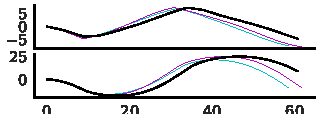
\includegraphics[]{figures/results_optiwise_ID.closed loop zigzag 10_10 port.pdf}
        \caption{Zigzag10/10 to port.}
        \label{fig:sim_optiwise_10_port}
     \end{subfigure}
     \hfill
     \begin{subfigure}[b]{0.49\textwidth}
         \includesvg{figures/results_optiwise_ID.closed loop zigzag 10_10 stbd.svg}
         %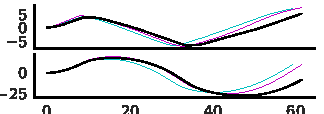
\includegraphics[]{figures/results_optiwise_ID.closed loop zigzag 10_10 stbd.pdf}
        \caption{Zigzag10/10 to starboard.}
        \label{fig:sim_optiwise_10_stbd}
     \end{subfigure}
     \vfill
     \begin{subfigure}[b]{0.49\textwidth}
         \centering
         \includesvg{figures/results_optiwise_ID.closed loop zigzag 20_20 port.svg}
         %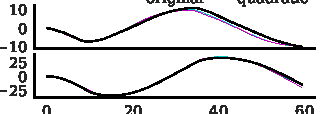
\includegraphics[]{figures/results_optiwise_ID.closed loop zigzag 20_20 port.pdf}
        \caption{Zigzag20/20 to port.}
        \label{fig:sim_optiwise_20_port}
     \end{subfigure}
     \hfill
     \begin{subfigure}[b]{0.49\textwidth}
         \includesvg{figures/results_optiwise_ID.closed loop zigzag 20_20 stbd.svg}
         %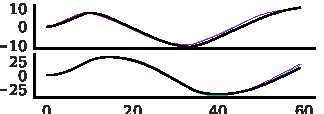
\includegraphics[]{figures/results_optiwise_ID.closed loop zigzag 20_20 stbd.pdf}
        \caption{Zigzag20/20 to starboard.}
        \label{fig:sim_optiwise_20_stbd}
     \end{subfigure}
     
        \caption{Comparison of zigzag tests between Optiwise experiments (black) and simulations with the MMG original (cyan) and MMG quadratic (purple).}
        \label{fig:sim_optiwise}
\end{figure}
%\input{kappa/04.10_discussion}





